\documentclass[14pt]{extarticle}

\usepackage{geometry}
\usepackage{amsmath,amsthm,amssymb}
\usepackage[utf8]{inputenc}
\usepackage[T1,T2A]{fontenc}
\usepackage{bold-extra}
\usepackage[english,russian]{babel}
\usepackage{indentfirst}
\usepackage{graphicx}
\graphicspath{ {images/} }
\usepackage{float}
\usepackage{listings}
\usepackage{lmodern}
\usepackage{appendix}
\usepackage{braket}
\usepackage{cite}
\usepackage[nottoc,numbib]{tocbibind}

\geometry{
a4paper,
left = 20mm,
right = 15mm,
bottom = 20mm,
top = 20mm,
}
\renewcommand{\rmdefault}{ftm} % TimesNewRoman
\renewcommand{\baselinestretch}{1.5} 

\begin{document}

\begin{titlepage}
	\begin{center}
		\small{ФЕДЕРАЛЬНОЕ ГОСУДАРСТВЕННОЕ БЮДЖЕТНОЕ ОБРАЗОВАТЕЛЬНОЕ}\\ 
			УЧРЕЖДЕНИЕ ВЫСШЕГО ОБРАЗОВАНИЯ\\
			«МОСКОВСКИЙ ГОСУДАРСТВЕННЫЙ УНИВЕРСИТЕТ\\
			имени М.В.ЛОМОНОСОВА»\\
		\hfill \break
		ФАКУЛЬТЕТ ВЫЧИСЛИТЕЛЬНОЙ МАТЕМАТИКИ И КИБЕРНЕТИКИ\\
		КАФЕДРА СУПЕРКОМПЬЮТЕРОВ И КВАНТОВОЙ ИНФОРМАТИКИ\\
		\vfill
		ЗАДАНИЕ 4 \\
		\textbf{<<АНАЛИЗ ПАРАЛЛЕЛЬНОГО АЛГОРИТМА УМНОЖЕНИЯ МАТРИЦЫ НА ВЕКТОР>>}\\
	\end{center}	
	\vfill
	\begin{flushright}
		Выполнил студент \\
		группы м118:\\
		Пухов Д. Н.\\
		{\hspace{3cm}}
	\end{flushright}
	
	
	\begin{center}
		Москва \\
		2018
	\end{center}
	
	\thispagestyle{empty}

\end{titlepage}

\tableofcontents
\newpage



\section{Формулировка задачи}
Реализовать параллельный алгоритм умножения матрицы на вектор, рассмотрев разбиение матрицы блоками строк и блоками столбцов в зависимости от входных данных. Найти теоретические и экспериментальные зависимости времени работы программы от числа используемых процессоров, размера входных данных, мэппинга процессов по процессорам. Дополнить отчёт соответствующими графиками, а именно: время работы, ускорение, эффективность программы. Также заполнить таблицу, чтобы резюмировать отчёт.

\section{Описание алгоритма}
Уравнение $ c = A \cdot b $, где $ A = n \times m $, $ B = m \times 1 $, $ C = n \times 1 $, можно переписать следующим образом:
\begin{equation*}
c_{i} = \sum \limits_{k=0}^{k=m-1} a_{ik} b_{k}, \quad i = \overline{0,n-1},
\end{equation*}
что соответствует следующему коду на языке C (вектор $c$ считается обнулённым):
\begin{lstlisting}[language=C]
for(int i=0; i<n; ++i)
	for(int k=0; k<m; ++k)
		c[i] += A[i][k] * b[k];
\end{lstlisting}

Ресурс параллелизма здесь очевиден --- компоненты вектора $c$ могут быть вычислены независимо. Достаточно распределить строки матрицы $A$ по процессорам, передав вектор $b$ каждому процессору целиком. Остаётся скопировать все части вектора $c$ на один процессор, и задача решена.

Однако, эту задачу можно разделить на подзадачи и другим способом. Каждый процессор будет хранить несколько столбцов матрицы $A$ и ровно столько же элементов вектора $b$. Тогда каждый процессор сможет вычислить свой вектор $c'$, сумма которых и будет результатом матричного умножения.

Существует и другой вариант --- распределение матрицы $A$ по процессорам блоками. Данный алгоритм не рассматривается.

\subsection{Деление задач по процессорам}
Для дальнейшего изложения рассмотрим вспомогательный алгоритм: как наиболее равномерно распределить некоторое количество равноценных заданий по некоторому числу равномощных процессоров.

Скажем, имеется два процессора. Два задания распределяются очевидным образом --- по одному на процессор. Три задания равномерно распределить невозможно. Сначала мы раздаём два задания (по одному, т.е. равномерно загружаем процессоры), затем выдаём третье, причём нет никакой разницы, какой процессор его получит. Четыре задания распределяются так же, как и два: поровну. Далее всё очевидно.

В случае трёх процессоров ситуация интереснее. Три задания распределяются поровну, четыре и пять заданий --- нет. Распределив три задания, четвёртое можно отдать любому процессору. А пятое --- уже не любому, нужно выбирать из тех, у кого по одному заданию. Действуя аналогично, можно распределить любое количество заданий. Заметим, что четыре задания можно распределить и иным способом: по два на первые два процессора, третий процессор простаивает. Ясно, что время работы будет таким же, как и в случае указанного ранее распределения. Посколько это распределение не имеет преимуществ, оно не рассматривается.

Программная реализация этого алгоритма на языке C принимает число заданий, число процессоров и адреса, по которым нужно поместить указатели на векторы, описывающие, сколько заданий выполняет процесс, номер первого задания и номер следующего за последним задания. Например, для трёх процессоров и пяти задач результат такой: первый процесс берёт два задания, с нулевого до второго (не включая), второй процесс берёт два задания, со второго по четвёртое, пятый --- одно задание, под номером четыре.

\begin{lstlisting}[language=C]
void distribute_tasks(int n_tasks, int n_proc, int **tasks_ptr,
                      int **from_ptr, int **to_ptr)
{
    // max tasks per process
    const int tpp = (n_tasks-1)/n_proc + 1;
    const int remained = n_tasks - (tpp-1)*n_proc;
    const int min_task_quantity = (tpp > 0 ? tpp-1 : 0);
    *tasks_ptr = safe_malloc(n_proc*sizeof(int));
    int * const tasks = *tasks_ptr;
    for(int i=0; i<n_proc; ++i) tasks[i] = min_task_quantity;
    for(int i=0; i<remained; ++i) ++tasks[i];

    *from_ptr = malloc(n_proc*sizeof(int));
    *to_ptr = malloc(n_proc*sizeof(int));
    int * const from = *from_ptr;
    int * const to = *to_ptr;
    from[0] = 0;
    to[0] = tasks[0];
    for(int i=1; i<n_proc; ++i)
    {
        from[i] = to[i-1];
        to[i] = from[i] + tasks[i];
    }
}
\end{lstlisting}

\subsection{Разбиение по строкам}
Стратегию разбиения по строкам следует применять в случае, когда число строк матрицы $A$ больше числа рядов этой матрицы.

Распределение задач по процессорам получаем с помощью процедуры \\ $distribute\_tasks()$, где числом заданий будет число строк. Для сбора информации используем процедуру $MPI\_Gatherv()$, которая разрешает отправку массивов разного размера.

Алгоритмическая часть программы выглядит следующим образом:

\begin{lstlisting}[language=C]
for(int i=0; i<tasks[rank]; ++i)
{
    const int i_n = i*n;
    double ci = 0.0;
    for(int k=0; k<n; ++k)
        ci += A[i_n+k] * b[k];
    c[i] = ci;
}
MPI_Gatherv(c, tasks[rank], MPI_DOUBLE, recvbuf, tasks, from,
			MPI_DOUBLE, 0, MPI_COMM_WORLD);
\end{lstlisting}

Здесь $c$ --- вектор длины $tasks[rank]$, который будет скопирован в по адресу $recvbuf$ в память процесса 0 (мастер-процесса). Матрица $A$ хранится построчно в одномерном массиве.

\subsection{Разбиение по столбцам}
Применяется, когда число столбцов больше числа строк.

Число заданий --- число столбцов. Для сбора информации используем процедуру $MPI\_Reduce()$, которая выполнит сложение векторов, хранящихся на разных процессорах.

\begin{lstlisting}[language=C]
// number of coloumns
const int n_tasks = tasks[rank];
for(int i=0; i<m; ++i)
{
    const int i_offset = i*n_tasks;
    double ci = 0.0;
    for(int k=0; k<n_tasks; ++k)
        ci += A[i_offset+k] * b[k];
    c[i] = ci;
}
MPI_Reduce(c, recvbuf, m, MPI_DOUBLE, MPI_SUM, 0,
           MPI_COMM_WORLD);
\end{lstlisting}

\subsection{Измерение времени}
Измерялось время выполнения алгоритмической части кода (приведён выше) с усреднением по пяти запускам (одно и то же вычисление просто запускалось в цикле, на тех же данных). Затем выбиралось максимальное среди процессоров время и выводилось в файо. Также в некоторых запусках измерялось время работы функции сбора информации ($MPI\_Gatherv()$ или $MPI\_Reduce()$).

Для измерения времени использовалась функция $clock()$ библиотеки $<time.h>$, которая возвращает время работы процессора начиная с некоторого момента в прошлом, не включая моменты простаивания. Правильней было бы использовать функцию $MPI_Wtime()$, которая возвращает время, прошедшее с некоторого момента в прошлом, посколько при осуществлении коммуницации между процессорами процессоры могут простаивать. Было проведено одно измерение с помощью обеих функций --- разница в результатах не обнаружена, так что можно полагаться на верность функции $clock()$.

\section{Описание программы}
\subsection{Запуск}
Для постановки задачи в очередь достаточно ввести make run. Makefile содержит следующие параметры:
\begin{itemize}
\item $NNODES$ --- число требуемых процессоров (до 32) или узлов (от 32)
\item $MAP$ --- режим работы узлов ($SMP$, $DUAL$, $VN$)
\item $MAPPING$ --- тип мэппинга процессов на процессоры ($XYZT$, $TXYZ$ и т.д.). Для случайного мэппинга требуется указать имя файла с координатами процессоров. Он генерируется командой $make map$ и название хранится в переменной $MAPFILE$. Также переменной мэппинг рекомендуется присвоить имя $RAND$ для корректного вывода
\item $M$, $N$ --- число строк и столбцов матрицы
\end{itemize}

\subsection{Формат вывода данных}
Для каждого запуска вывод данных происходит в файл  \\ $../out/\$(MAP).\$(MODE).\$(M).\$(N).\$(NNODES).out$ и имеет вид:
\begin{lstlisting}
n_proc: 512
matrix: 4096x4096
row blocked
MPI time: 0.340000
\end{lstlisting}

\subsection{Формат записи матриц в файл}
Матрицы хранятся построчно в бинарном виде в следующем формате:
\begin{itemize}
\item $type(int)$ --- формат данных (0 --- $float$, 1 --- $double$)
\item $m(int), n(int)$ --- число строк и столбцов матрицы
\item элементы матрицы
\end{itemize}

\subsection{Обработка результатов}
Для обработки на домашней машине предусмотрена команда make report, которая запустит скрипт на языке python и построит по одному графику для каждого режима работы узлов (для построения графиков эффективности и ускорения необходимо внести небольшие изменения в код файла report.py). Требуются файлы из папки $../res$.

\section{Результаты}
В задаче исследуется сильная масштабируемость --- зависимость времени работы программы при фиксированных входных от числа используемых процессоров. На системе Blue Gene\textbackslash P предусмотрены несколько сетей для связи узлов: тор (от 512), дерево и некая коллективная сеть для прерываний типа $MPI\_Barrier()$. В задаче использовалось до 256 узлов, причём прерывания не были использованы в измеряемых частях код. Так что можно заключить, что топология связи процессоров --- дерево, с характерной асимптотикой времени работы $log_2(n\_nodes)$.

\subsection{SMP режим}
В этом режиме каждый MPI процесс привязан к нулевому процессору соответствующего узла, процессоры 1, 2, 3 простаивают (они могут быть использованы для создания нитей).

\begin{figure}[H]
	\centering
	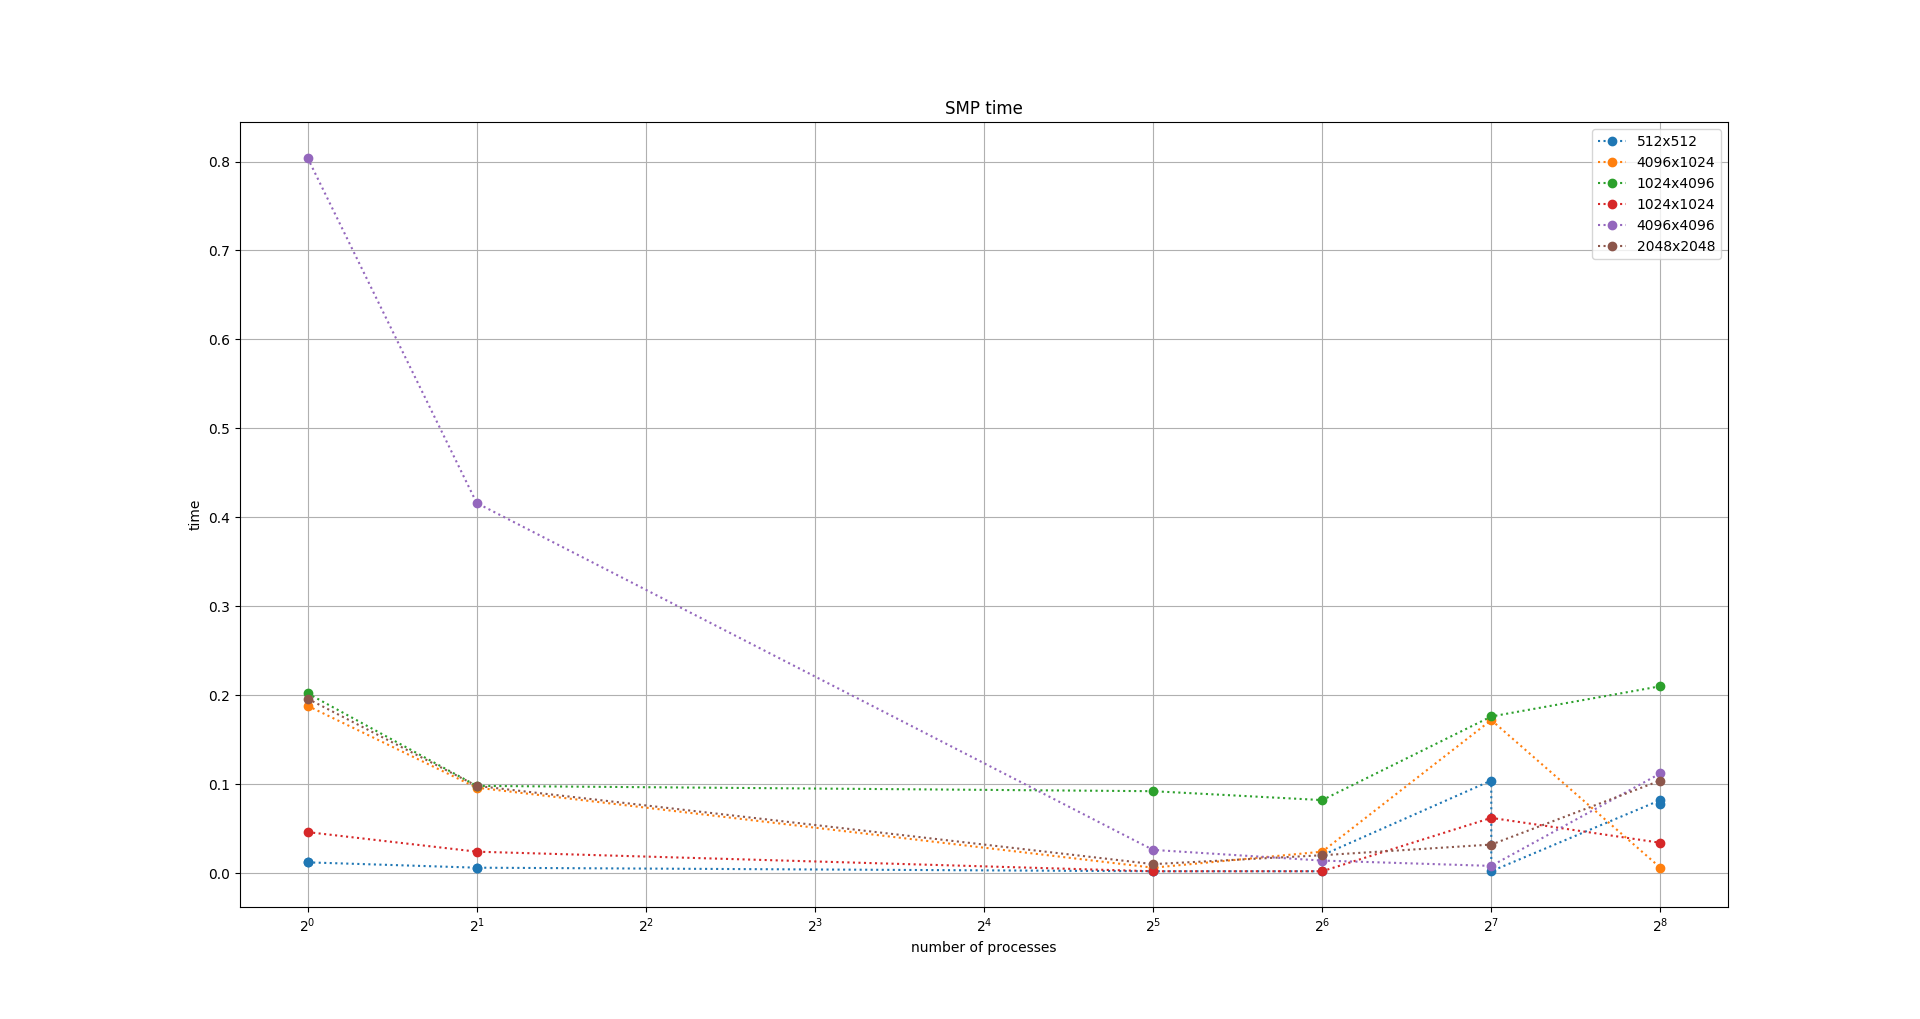
\includegraphics[scale=0.4]{SMP_time}
\end{figure}

\begin{figure}[H]
	\centering
	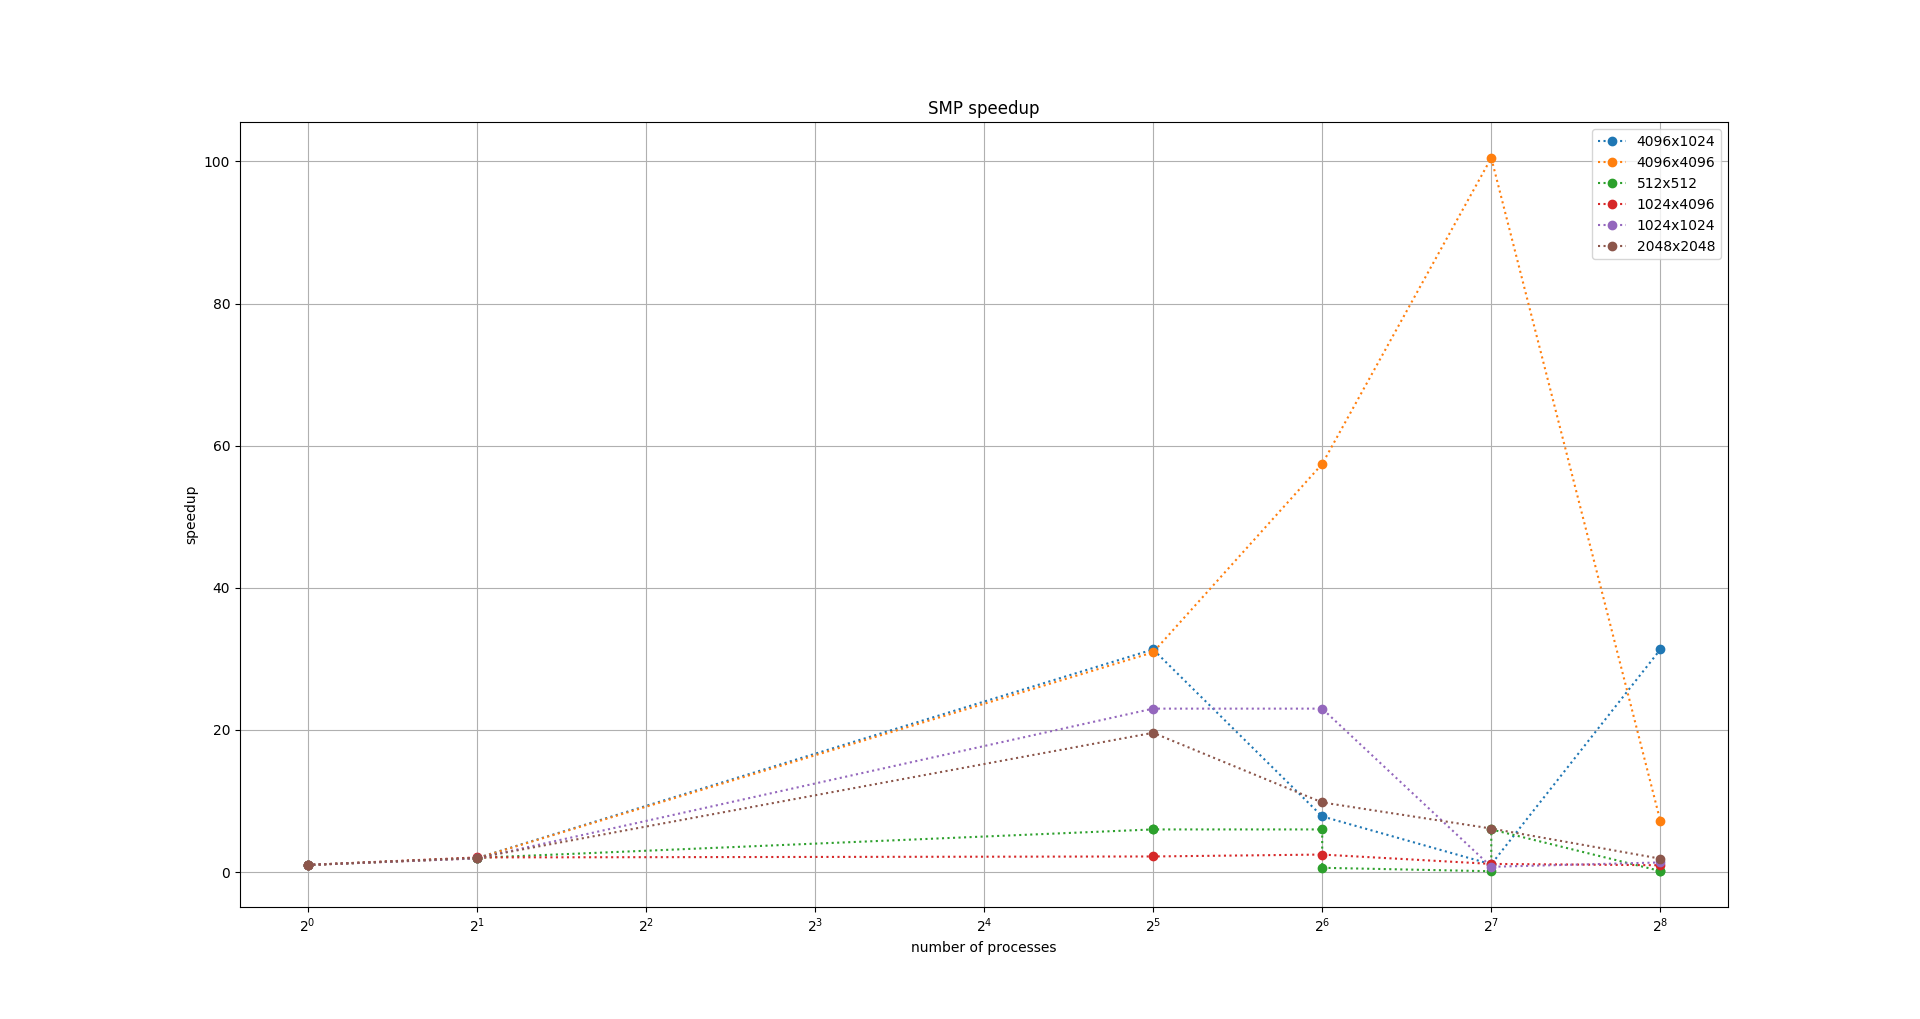
\includegraphics[scale=0.4]{SMP_speedup}
\end{figure}

\begin{figure}[H]
	\centering
	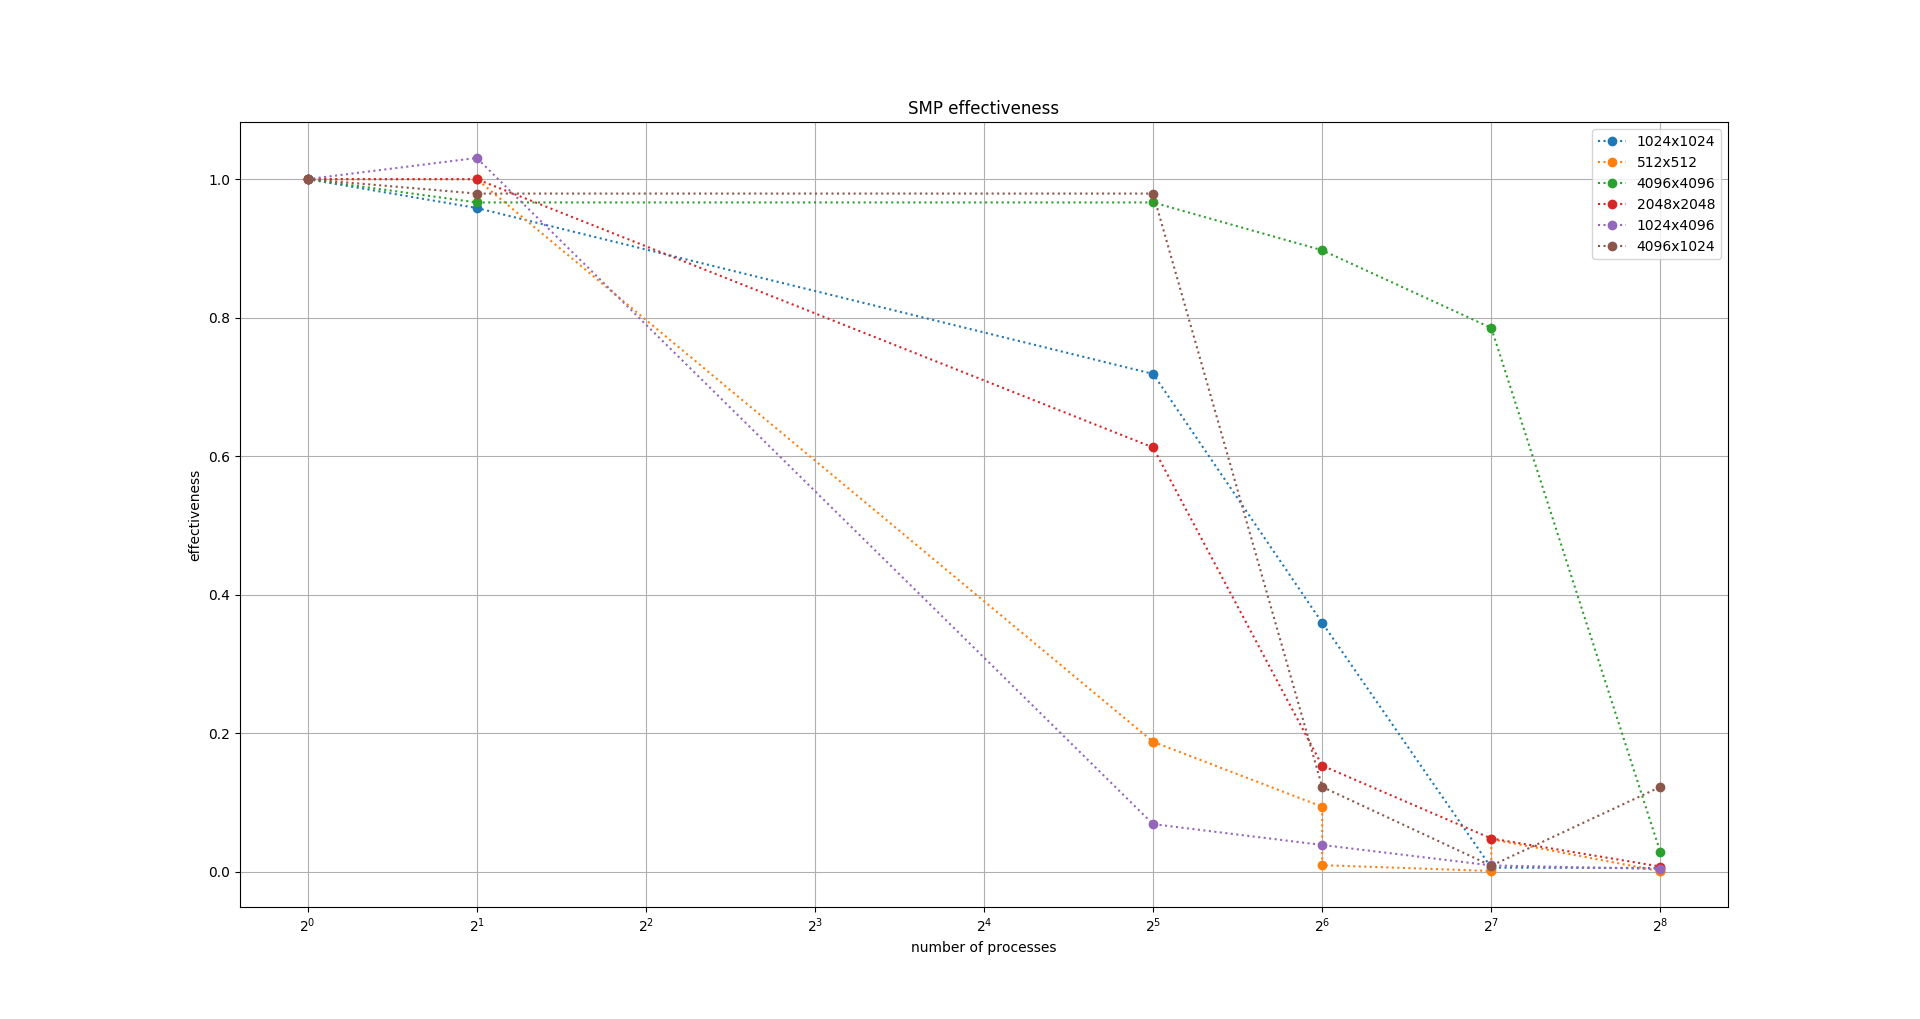
\includegraphics[scale=0.4]{SMP_effectiveness}
\end{figure}

По первому графику видно, что время задачи хорошо масштабируются до двух процессоров, плохо до 32 и возникают отрицательный эффект от использования 256 процессоров: задача выполнется дольше, чем на 1 процессоре. Наилучшую масштабируемость можно наблюдать при максимальном размере задаче ($4096 \times 4096$), наихудшую --- при размере $1024 \times 4096$. Найти объяснение второму результату не удалось (возможно, плохая масштабируемость связана с необходимостью суммировать вектора). Дополнительно измерив время работы коллективных операций в алгоритмической части кода, можно заметить, что время работы программы при большом числе процессов на $99...100\%$ состоит из передачи сообщений. Это легко объясняется тем, что размер подзадач достаточно мал: при 32 процессорах одному процессору нужно произвестви обработку не более $\frac{4096}{32}=128$ строк или столбцов длиной не более 4096, что составляет около 1 миллиона операций с плавающей запятой, что при использовании одного ФУ для обработки чисел займёт 1 миллисекунду. Вопрос сводится к наиболее удачному размещению процессов по процессорам (здесь не рассматривается).

\subsection{DUAL режим}
В этом режиме на одном узле запускаются 2 MPI процесса, процессоры 1, 3 простаивают (они могут быть использованы для создания нитей).

Вертикальные линии на графиках означают использования разного мэппинга для одной задачи. Как можно видеть, мэппинг влияет на время выполнения программы только тогда, когда программа работает эффективно (при использовании 512 процессов точки видно только на графике времени).

\begin{figure}[H]
	\centering
	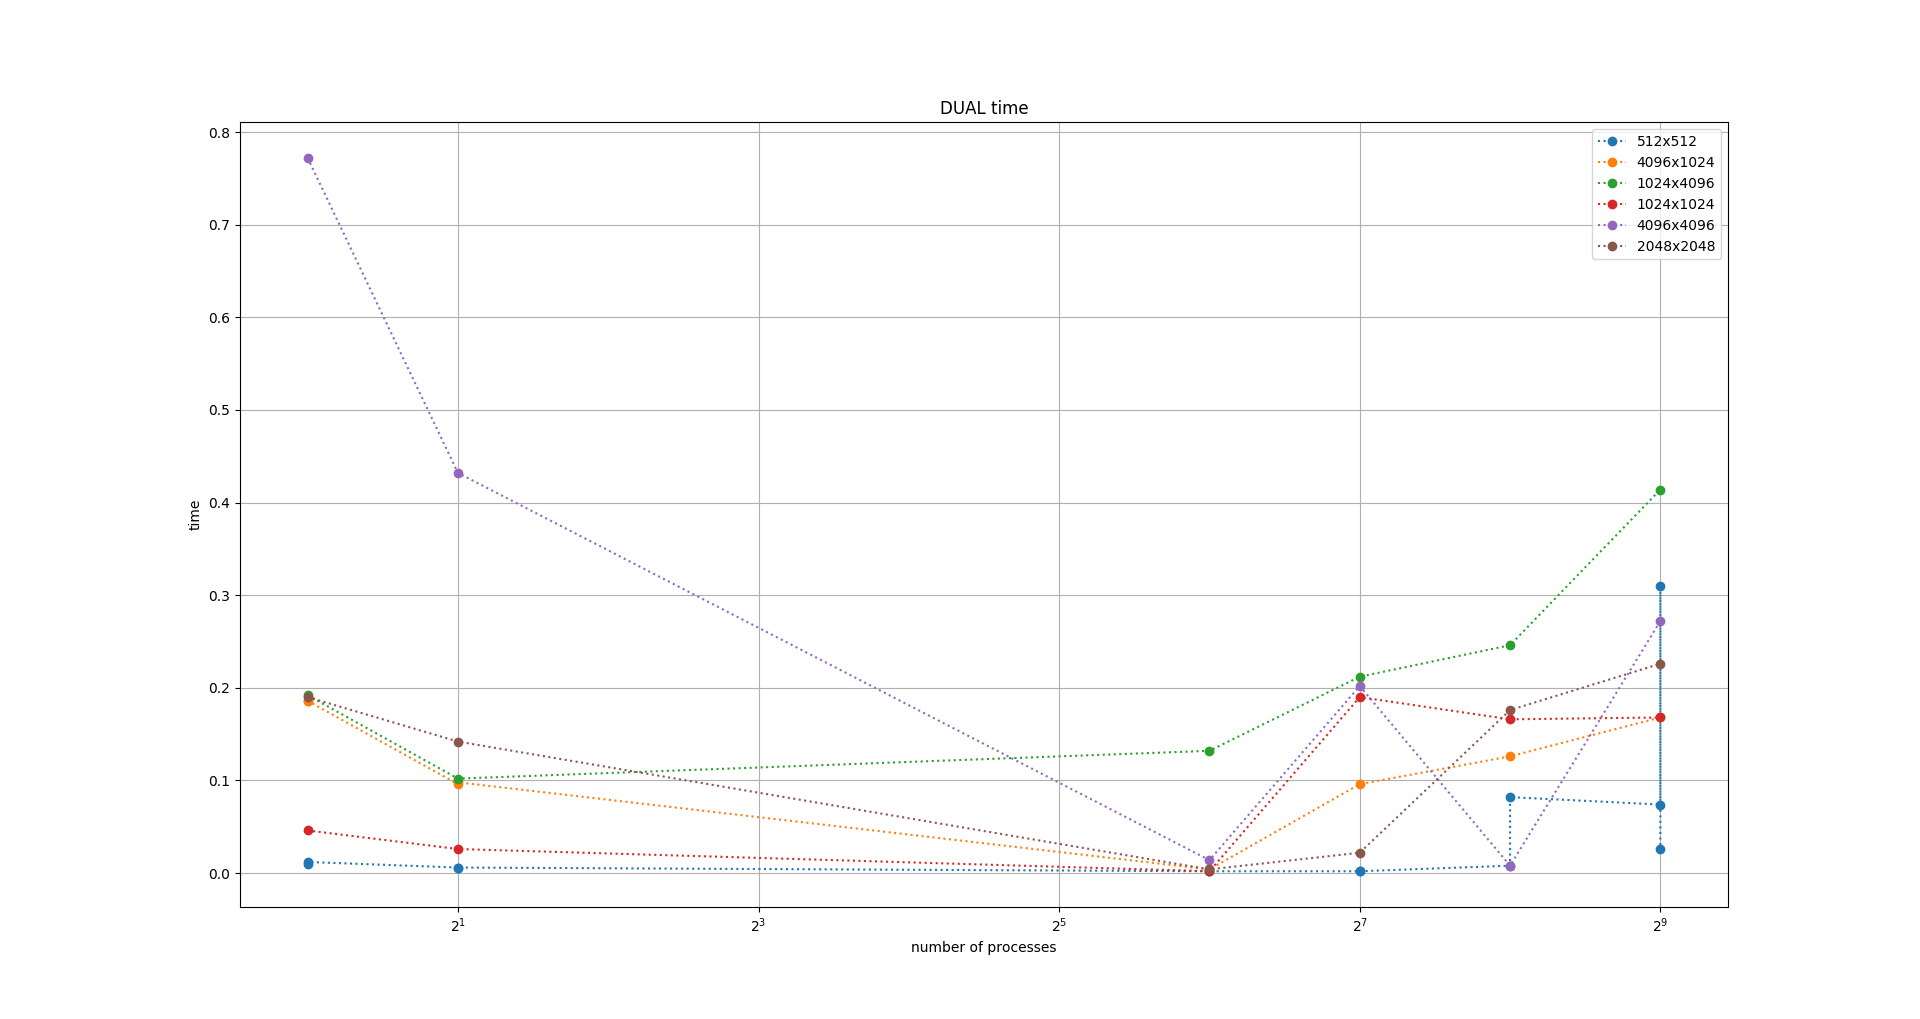
\includegraphics[scale=0.4]{DUAL_time}
\end{figure}

\begin{figure}[H]
	\centering
	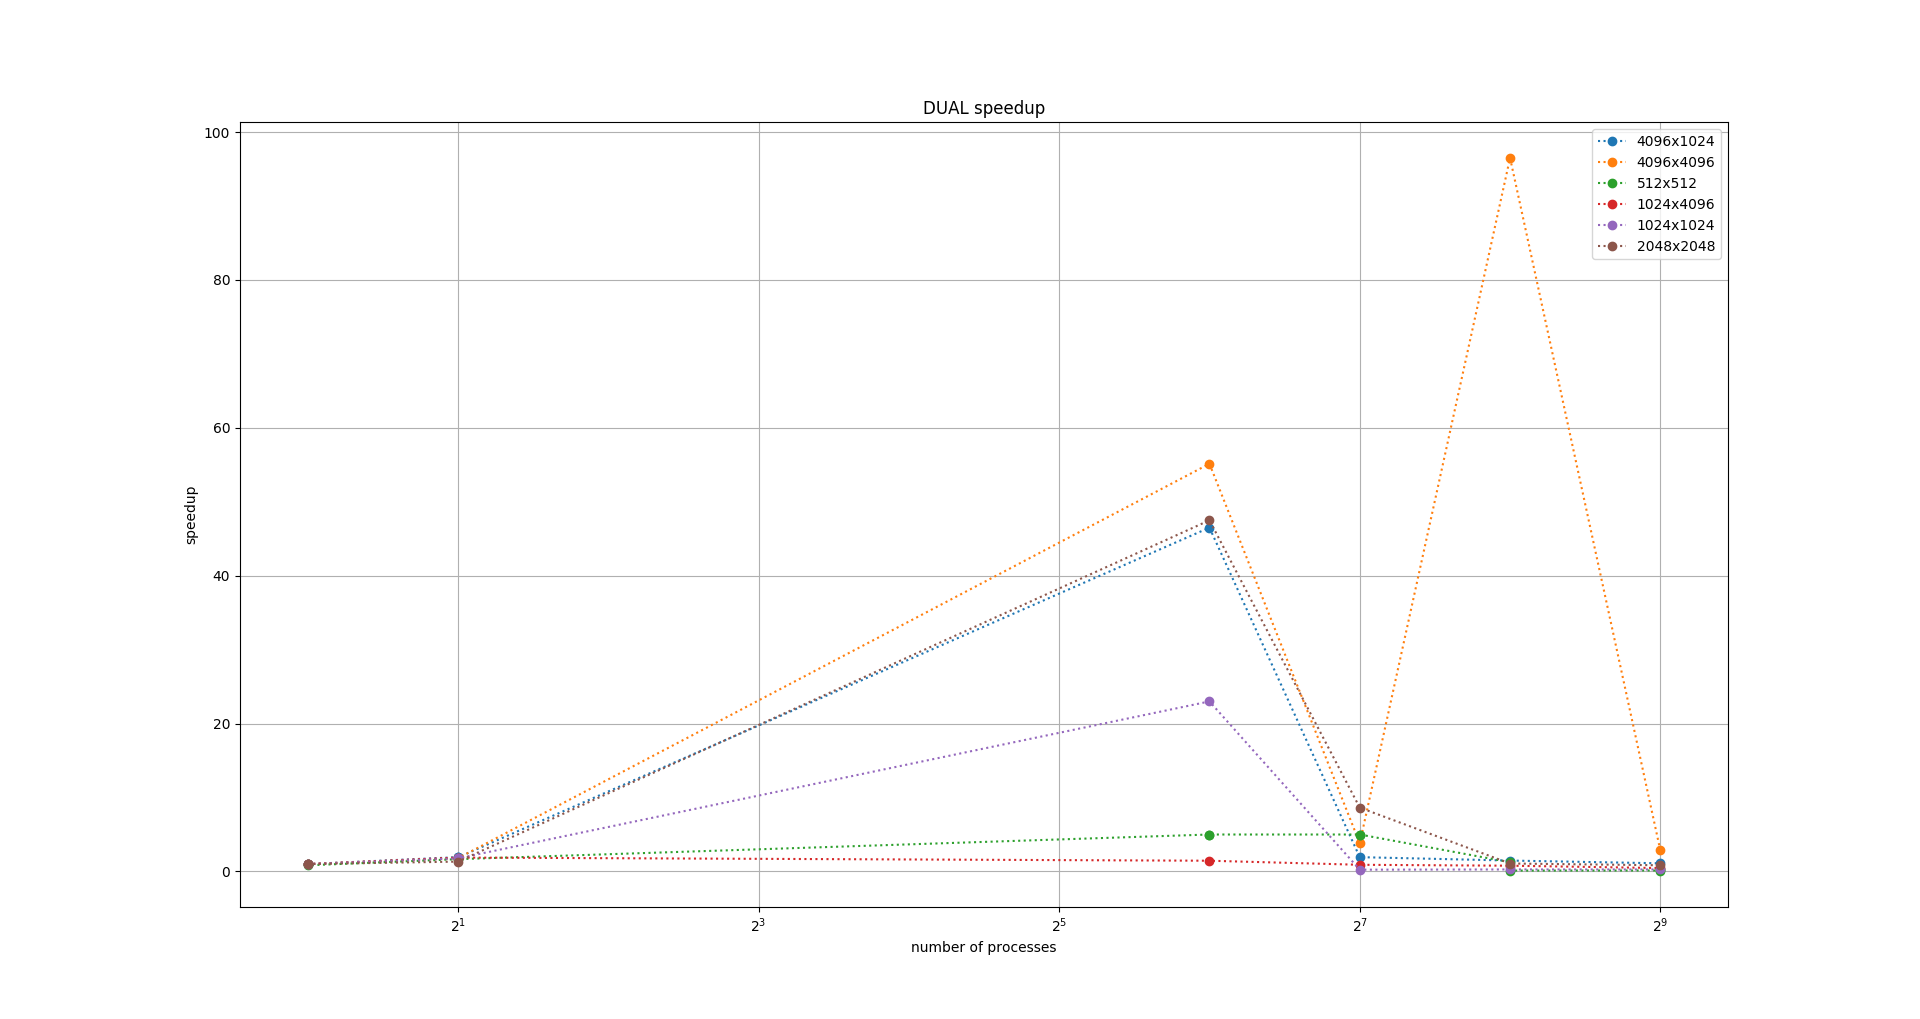
\includegraphics[scale=0.4]{DUAL_speedup}
\end{figure}

\begin{figure}[H]
	\centering
	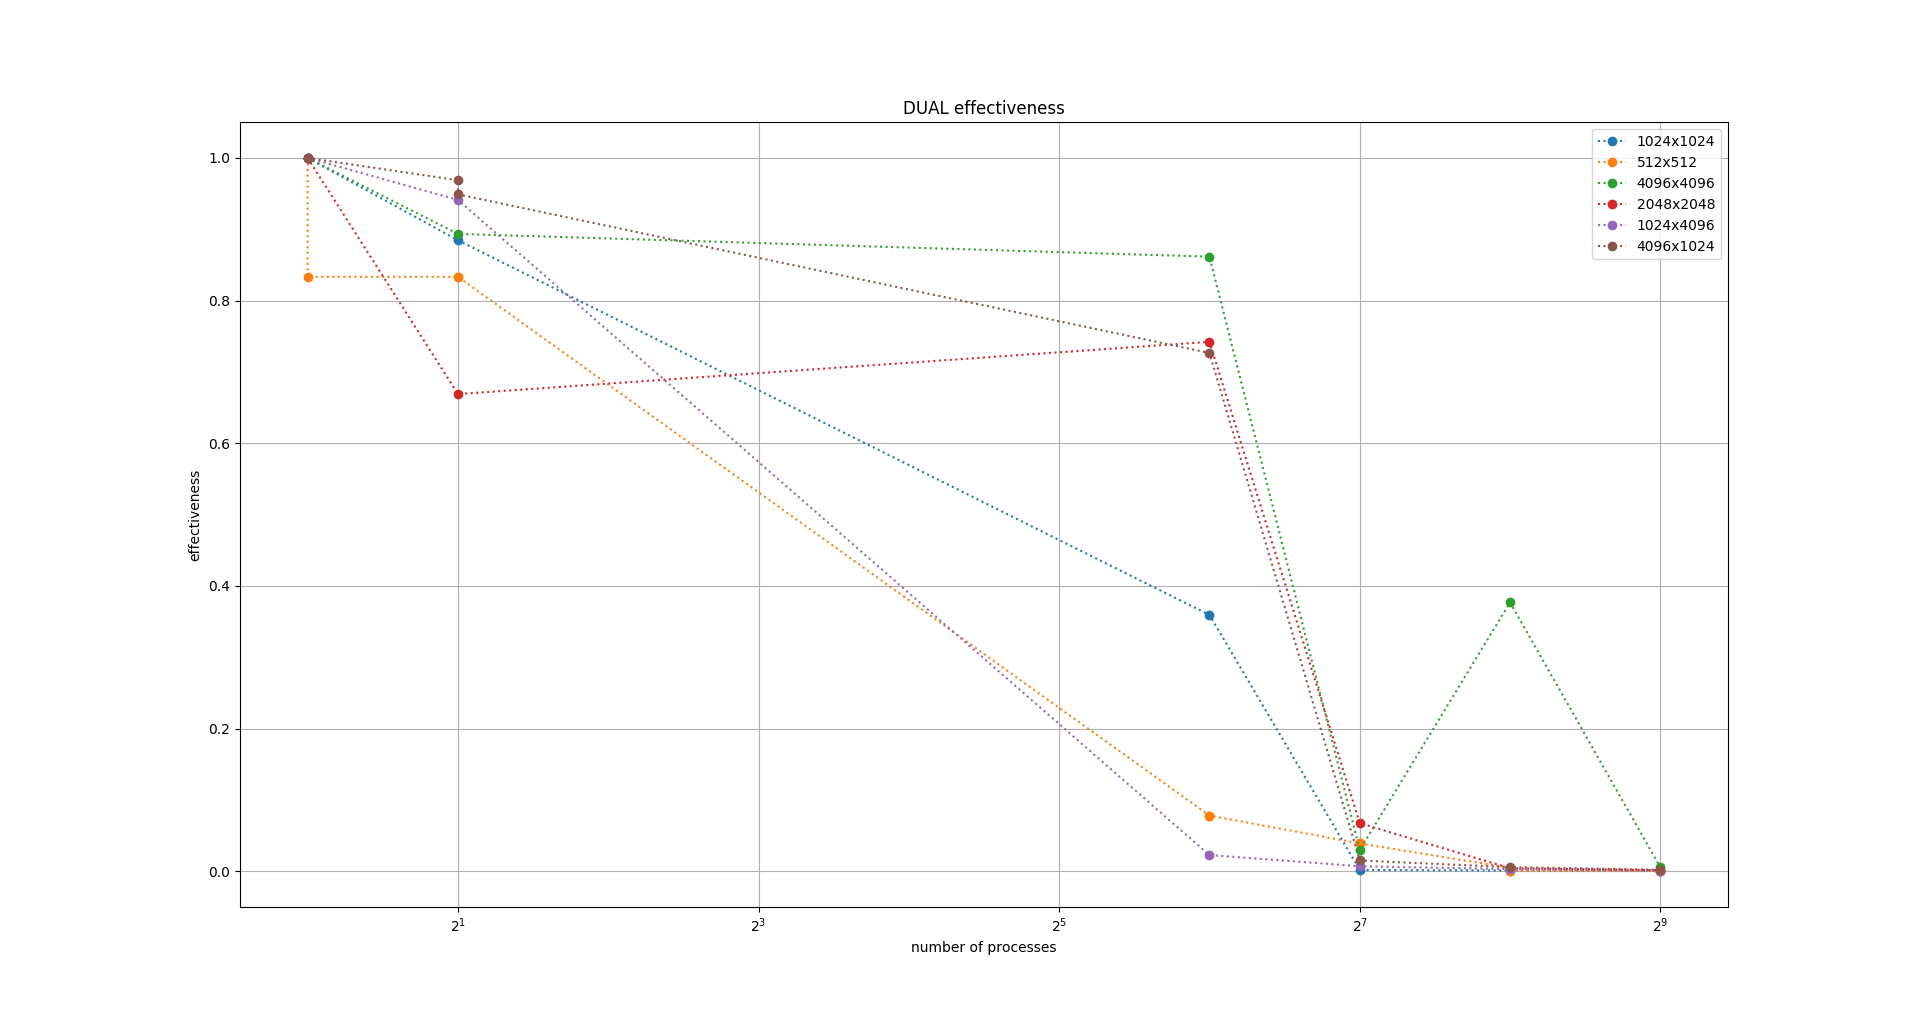
\includegraphics[scale=0.4]{DUAL_effectiveness}
\end{figure}

\subsection{VN режим}
В этом режиме все четыре процесса каждого узла могут быть использованы для размещения MPI процесса.

Для случая 512 процессов наряду со стандартным мэппингом использовался случайный мэппинг, сгенерированный командой make map. Обнаружить результат можно на графике времени. Так как программа работает крайне неэффективно, то на графиках эффективности и ускорения эти точки сливаются в одно пятно.

\begin{figure}[H]
	\centering
	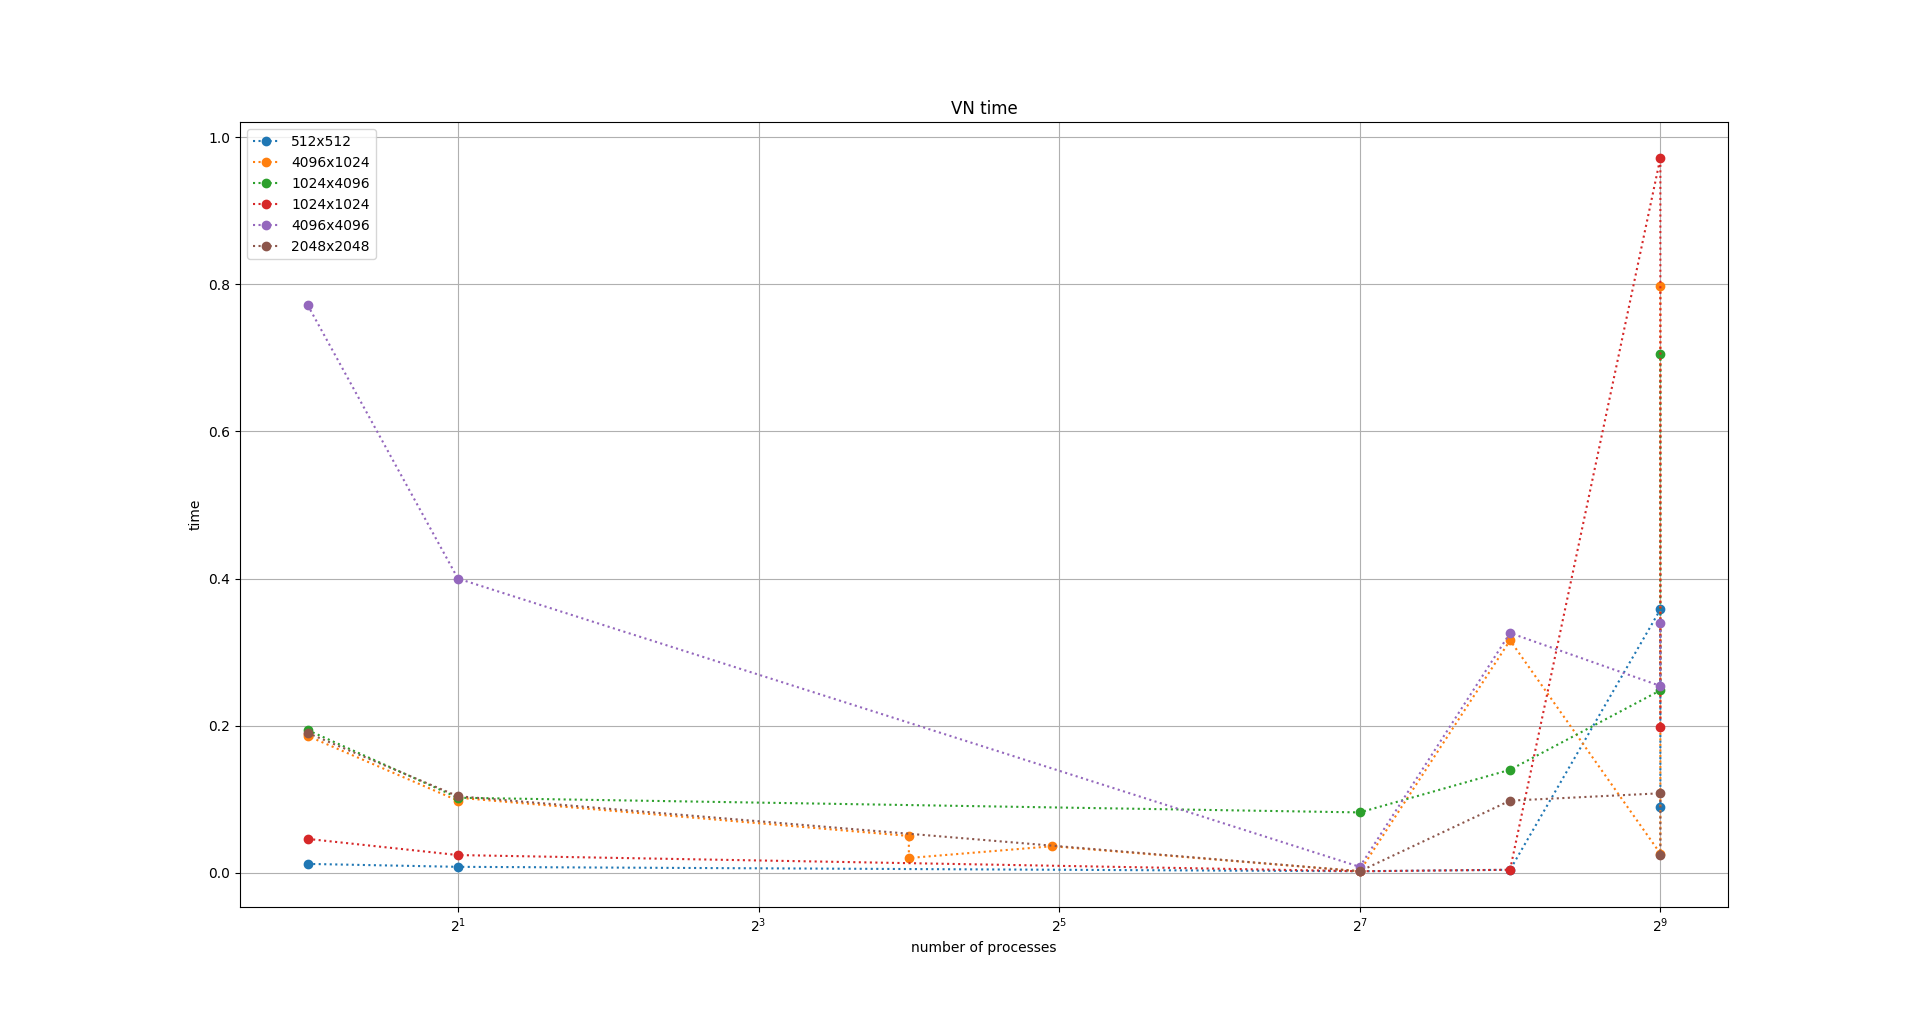
\includegraphics[scale=0.4]{VN_time}
\end{figure}

\begin{figure}[H]
	\centering
	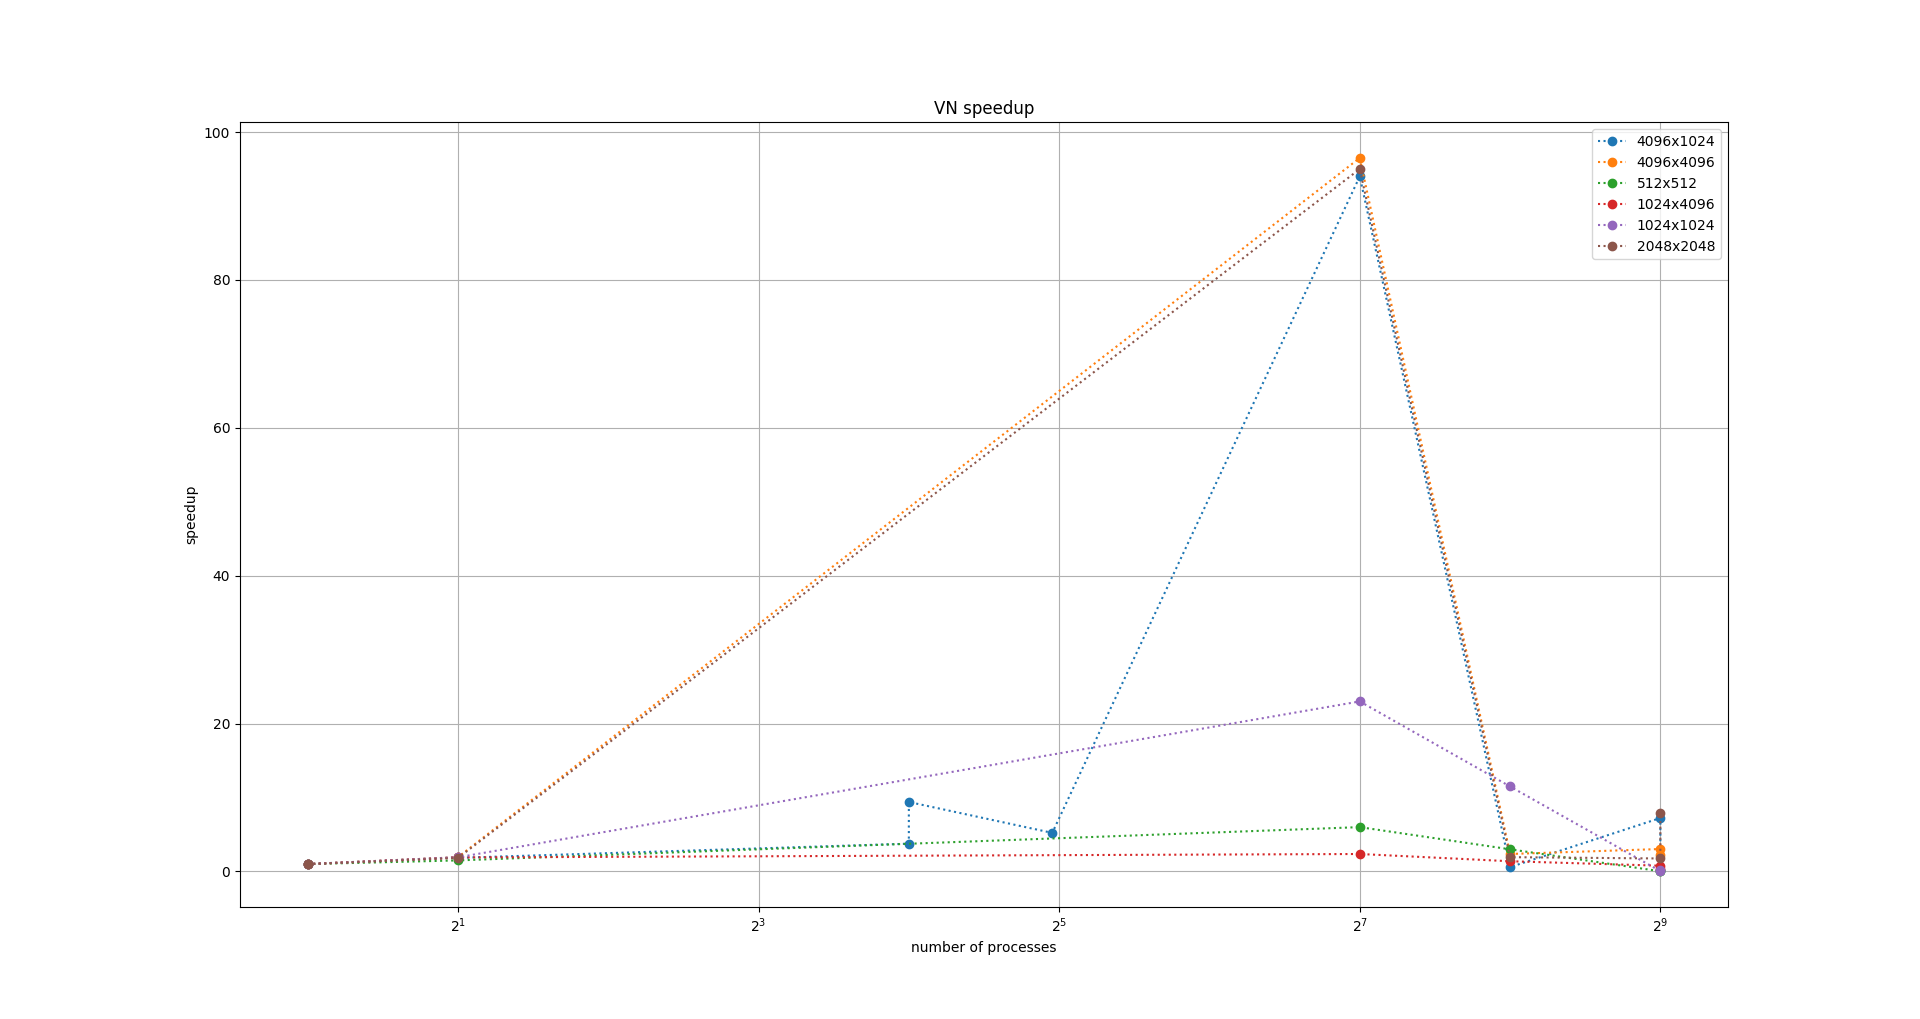
\includegraphics[scale=0.4]{VN_speedup}
\end{figure}

\begin{figure}[H]
	\centering
	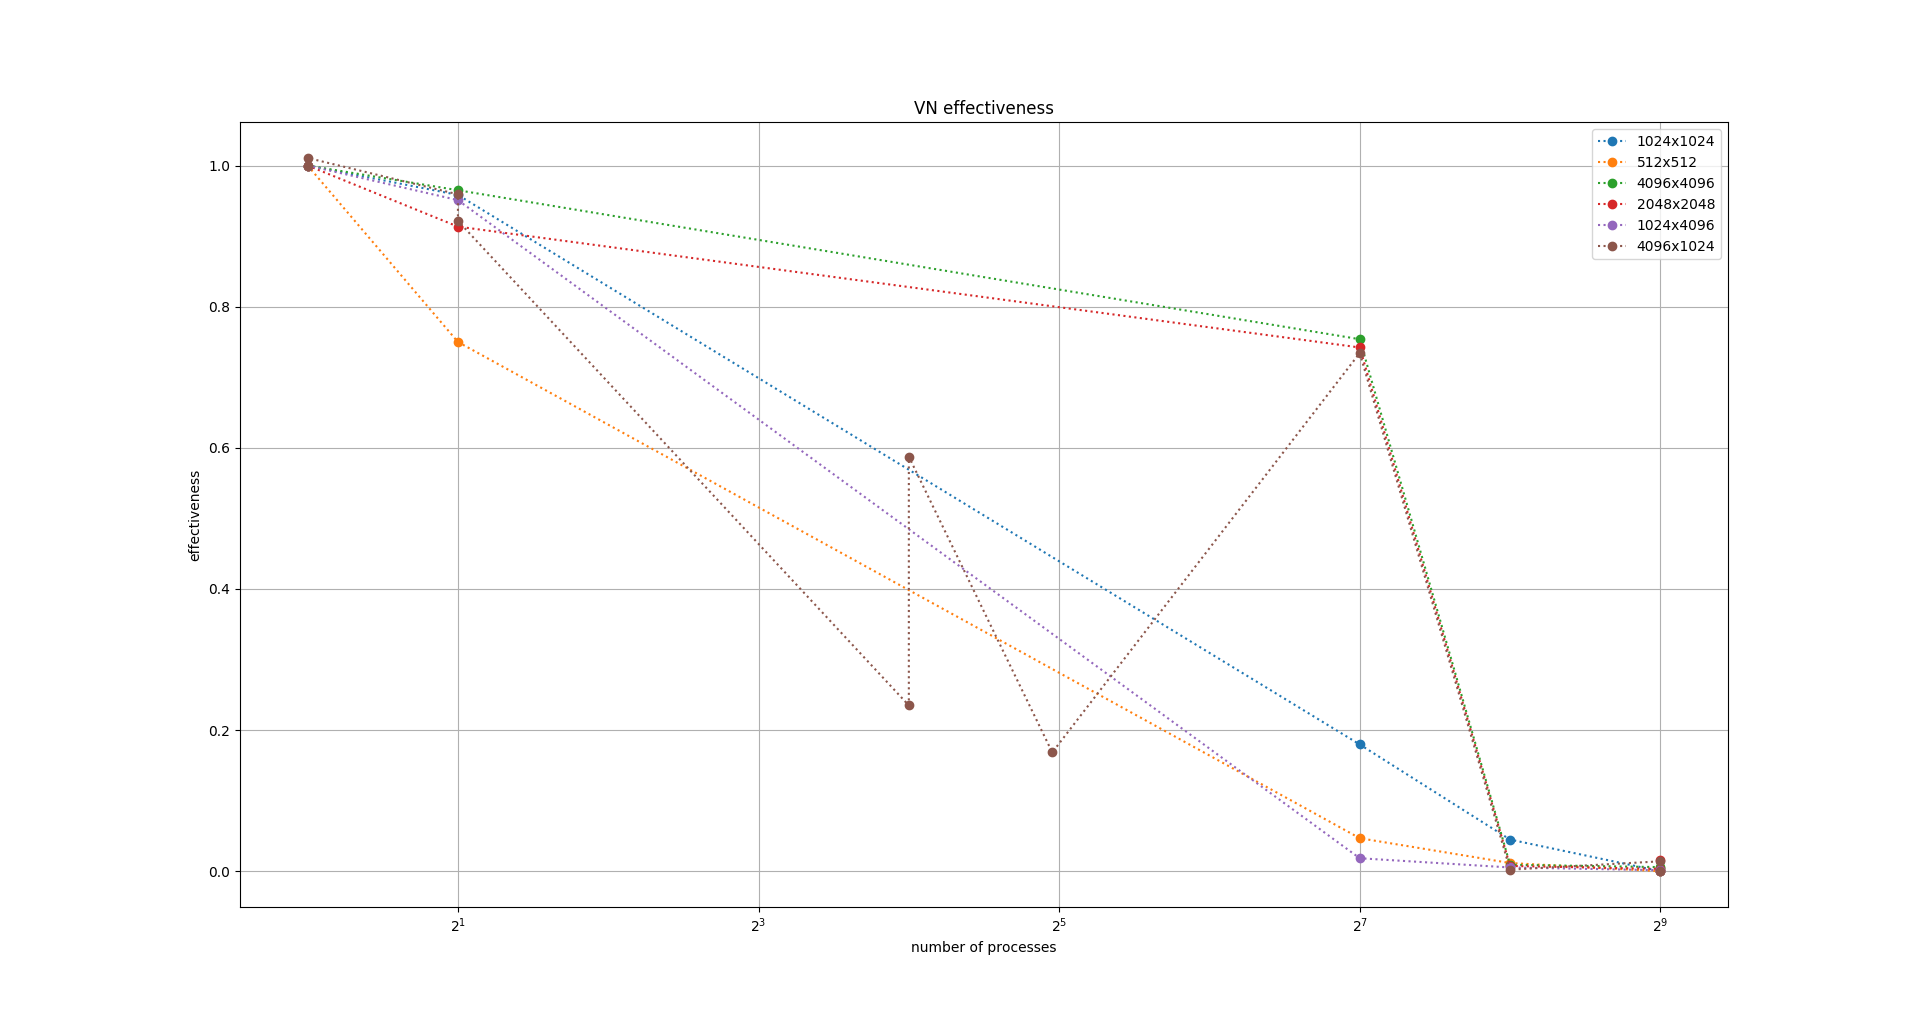
\includegraphics[scale=0.4]{VN_effectiveness}
\end{figure}

\end{document}\grid
